\documentclass[b0paper,margin=1cm,landscape]{baposter}

\usepackage{relsize}	       % For \smaller
\usepackage{url}			   % For \url
\usepackage{epstopdf}	       % Included EPS files automatically converted to PDF to include with pdflatex
\usepackage{multicol}          % Multi Columns

\usepackage{amsmath,amssymb}   % math
\usepackage{natbib}
\usepackage{graphicx}          % pix
\usepackage{xcolor}            % colurs
\usepackage{hyperref}          % linx

\definecolor{umblue}{rgb}{0.03, 0.15, 0.30}
\definecolor{ummaize}{rgb}{0.90, 0.85, 0.40}

%%%%%%%%%%%%%%%%%%%%%%%%%%%%%%%%%%%%%%%%%%%%%%%%%%%%%%%%%%%%%%%%%%%%%%%%%%%%%%%%%%%%%
%%% Utility functions %%%%%%%%%%%%%%%%%%%%%%%%%%%%%%%%%%%%%%%%%%%%%%%%%%%%%%%%%%%%%%%
%%%%%%%%%%%%%%%%%%%%%%%%%%%%%%%%%%%%%%%%%%%%%%%%%%%%%%%%%%%%%%%%%%%%%%%%%%%%%%%%%%%%%

%%%%%%%%%%%%%%%%%%%%%%%%%%%%%%%%%%%%%%%%%%%%%%%%%%%%%%%%%%%%%%%%%%%%%%%%%%%%%%%%%%%%%
%%% Save space in lists. Use this after the opening of the list %%%%%%%%%%%%%%%%%%%%%
%%%%%%%%%%%%%%%%%%%%%%%%%%%%%%%%%%%%%%%%%%%%%%%%%%%%%%%%%%%%%%%%%%%%%%%%%%%%%%%%%%%%%
\renewcommand{\vec}[1]{\bm{#1}}
\newcommand{\vnabla}{\vec{\nabla}}

\renewcommand{\d}[1]{\text{d} #1}
\newcommand{\dxx}{\,\text{d}\vec{x}}
\newcommand{\dx}{\,\text{d}x}

\newcommand{\diff}[2]{\frac{\text{d}#1}{\text{d}#2}}
\newcommand{\idiff}[2]{\text{d}#1 / \text{d}#2}
\newcommand{\pdiff}[2]{\frac{\partial #1}{\partial #2}}
\newcommand{\pdifff}[2]{\frac{\partial^2 #1}{\partial #2^2}}
\newcommand{\ipdiff}[2]{\partial #1 / \partial #2}
\newcommand{\vdiff}[2]{\frac{\delta #1}{\delta #2}}
\newcommand{\ivdiff}[2]{\delta #1 / \delta #2}

%%%%%%%%%%%%%%%%%%%%%%%%%%%%%%%%%%%%%%%%%%%%%%%%%%%%%%%%%%%%%%%%%%%%%%%%%%%%%%%%%%%%
%%% Document Start %%%%%%%%%%%%%%%%%%%%%%%%%%%%%%%%%%%%%%%%%%%%%%%%%%%%%%%%%%%%%%%%%
%%%%%%%%%%%%%%%%%%%%%%%%%%%%%%%%%%%%%%%%%%%%%%%%%%%%%%%%%%%%%%%%%%%%%%%%%%%%%%%%%%%%

\begin{document}
\typeout{Poster rendering started}

%%%%%%%%%%%%%%%%%%%%%%%%%%%%%%%%%%%%%%%%%%%%%%%%%%%%%%%%%%%%%%%%%%%%%%%%%%%%%%%%%%%%
%%% General Poster Settings %%%%%%%%%%%%%%%%%%%%%%%%%%%%%%%%%%%%%%%%%%%%%%%%%%%%%%%%
%%%%%% Eye Catcher, Title, Authors and University Images %%%%%%%%%%%%%%%%%%%%%%%%%%%
%%%%%%%%%%%%%%%%%%%%%%%%%%%%%%%%%%%%%%%%%%%%%%%%%%%%%%%%%%%%%%%%%%%%%%%%%%%%%%%%%%%%
\begin{poster}{
    columns=4,
    grid=false,
    borderColor=umblue,
    headerColorOne=umblue,
    headerColorTwo=umblue,
    headerFontColor=ummaize,
    headerheight=12em,
    boxColorOne=white,
    boxColorTwo=umblue,
    linewidth=1.5pt,
    boxpadding=0.66em,
    headershape=rectangle,
    headerfont=\Large\textsf,
    textborder=faded,
    background=plain,
    bgColorOne=white,
    bgColorTwo=umblue,
    headerborder=closed,
    boxshade=plain,
    headershade=plain,
    eyecatcher=false
}
%%%%%%%%%%%%%%%%%%%%%%%%%%%%%%%%%%%%%%%%%%%%%%%%%%%%%%%%%%%%%%%%%%%%%%%%%%%%%%%%%%%%
%%% Eye Catcher %%%%%%%%%%%%%%%%%%%%%%%%%%%%%%%%%%%%%%%%%%%%%%%%%%%%%%%%%%%%%%%%%%%%
%%%%%%%%%%%%%%%%%%%%%%%%%%%%%%%%%%%%%%%%%%%%%%%%%%%%%%%%%%%%%%%%%%%%%%%%%%%%%%%%%%%%
{
}
%%%%%%%%%%%%%%%%%%%%%%%%%%%%%%%%%%%%%%%%%%%%%%%%%%%%%%%%%%%%%%%%%%%%%%%%%%%%%%%%%%%%
%%% Title %%%%%%%%%%%%%%%%%%%%%%%%%%%%%%%%%%%%%%%%%%%%%%%%%%%%%%%%%%%%%%%%%%%%%%%%%%
%%%%%%%%%%%%%%%%%%%%%%%%%%%%%%%%%%%%%%%%%%%%%%%%%%%%%%%%%%%%%%%%%%%%%%%%%%%%%%%%%%%%
{Assessing the Ecology of the Flint River, Above and Below a Century-Old Dam}
%%%%%%%%%%%%%%%%%%%%%%%%%%%%%%%%%%%%%%%%%%%%%%%%%%%%%%%%%%%%%%%%%%%%%%%%%%%%%%%%%%%%
%%% Authors %%%%%%%%%%%%%%%%%%%%%%%%%%%%%%%%%%%%%%%%%%%%%%%%%%%%%%%%%%%%%%%%%%%%%%%%
%%%%%%%%%%%%%%%%%%%%%%%%%%%%%%%%%%%%%%%%%%%%%%%%%%%%%%%%%%%%%%%%%%%%%%%%%%%%%%%%%%%%
{
  \vspace{0mm}
  \text{Chloe Summers} : \textit{\color{violet}{summersj@umich.edu}}, 
  \text{Arianna Elkins} : \textit{\color{violet}{arelkins@umich.edu}}, 
  \text{Cason Konzer} : \textit{\color{violet}{casonk@umich.edu}}, 
  \text{Heather Dawson} : \textit{\color{violet}{hdawson@umich.edu}} 
  
  \hspace{1mm} $\downharpoonright$ website : \textit{\color{violet}{https://flintriverecostudy.com}}
  \hspace{1mm} $\downharpoonright$ repository : \textit{\color{violet}{https://github.com/casonk/Flint\_River\_Ecology}}
}
%%%%%%%%%%%%%%%%%%%%%%%%%%%%%%%%%%%%%%%%%%%%%%%%%%%%%%%%%%%%%%%%%%%%%%%%%%%%%%%%%%%%
%%% Logo %%%%%%%%%%%%%%%%%%%%%%%%%%%%%%%%%%%%%%%%%%%%%%%%%%%%%%%%%%%%%%%%%%%%%%%%%%%
%%%%%%%%%%%%%%%%%%%%%%%%%%%%%%%%%%%%%%%%%%%%%%%%%%%%%%%%%%%%%%%%%%%%%%%%%%%%%%%%%%%%
{
  \begin{minipage}{8.0em}
    
\includegraphics[height=8em]{Img/Ecology_Study.png}
  \end{minipage}
  \begin{minipage}{8.0em}
    
\includegraphics[height=8em]{Img/University_of_Michigan_Flint.png}
  \end{minipage}
}
%%%%%%%%%%%%%%%%%%%%%%%%%%%%%%%%%%%%%%%%%%%%%%%%%%%%%%%%%%%%%%%%%%%%%%%%%%%%%%%%%%%%
%%% Objective %%%%%%%%%%%%%%%%%%%%%%%%%%%%%%%%%%%%%%%%%%%%%%%%%%%%%%%%%%%%%%%%%%%%%%
%%%%%%%%%%%%%%%%%%%%%%%%%%%%%%%%%%%%%%%%%%%%%%%%%%%%%%%%%%%%%%%%%%%%%%%%%%%%%%%%%%%%
\headerbox{Objective}{name=box00, column=0, row=0}{\textbf{
  Investigate and collect data on the ecology and health of the Flint River 
  above and below the Hamilton Dam before removal to gain an understanding of the 
  present ecosystem and provide grounds for future research.}
}
%%%%%%%%%%%%%%%%%%%%%%%%%%%%%%%%%%%%%%%%%%%%%%%%%%%%%%%%%%%%%%%%%%%%%%%%%%%%%%%%%%%%
%%% Background %%%%%%%%%%%%%%%%%%%%%%%%%%%%%%%%%%%%%%%%%%%%%%%%%%%%%%%%%%%%%%%%%%%%%
%%%%%%%%%%%%%%%%%%%%%%%%%%%%%%%%%%%%%%%%%%%%%%%%%%%%%%%%%%%%%%%%%%%%%%%%%%%%%%%%%%%%
\headerbox{Background}{name=box01, column=0, row=1, below=box00}{
  \begin{itemize} \normalsize 
    \item The Hamilton Dam, constructed in 1920, resides in the urban 
    city of Flint, Michigan and was utilized for logging and the automobile industry.
    \item It no longer serves this purpose and is in the process of 
    removal to revert the stream to its natural ecology.
    \item Upstream reaches of the Hamilton dam consist of a wide riparian zone, 
    whereas downstream is composed of \\ cemented structures with trapped debris.
  \end{itemize}
}
%%%%%%%%%%%%%%%%%%%%%%%%%%%%%%%%%%%%%%%%%%%%%%%%%%%%%%%%%%%%%%%%%%%%%%%%%%%%%%%%%%%%
%%% Introduction %%%%%%%%%%%%%%%%%%%%%%%%%%%%%%%%%%%%%%%%%%%%%%%%%%%%%%%%%%%%%%%%%%%
%%%%%%%%%%%%%%%%%%%%%%%%%%%%%%%%%%%%%%%%%%%%%%%%%%%%%%%%%%%%%%%%%%%%%%%%%%%%%%%%%%%%
\headerbox{Introduction}{name=box02, column=0, row=1, below=box01}{
  \begin{itemize} \normalsize 
    \item Ecology study on the Flint River before the weir is \\ removed in 2023 
    through a \$33 million project to restore habitat and recreational utility.
    \item This data will later be compared to data collected once the weir 
    is removed to assess the impact of habitat \\ fragmentation and relay how 
    restoration efforts can affect riverine ecosystems.
    \item Multiple fishing methods were necessary to assess the varying 
    habitats upstream and downstream as a result of the dam.
  \end{itemize}
}
%%%%%%%%%%%%%%%%%%%%%%%%%%%%%%%%%%%%%%%%%%%%%%%%%%%%%%%%%%%%%%%%%%%%%%%%%%%%%%%%%%%%
%%% Methods %%%%%%%%%%%%%%%%%%%%%%%%%%%%%%%%%%%%%%%%%%%%%%%%%%%%%%%%%%%%%%%%%%%%%%%%
%%%%%%%%%%%%%%%%%%%%%%%%%%%%%%%%%%%%%%%%%%%%%%%%%%%%%%%%%%%%%%%%%%%%%%%%%%%%%%%%%%%%
\headerbox{Methods}{name=box03, column=0, row=1, above=bottom, below=box02}{
  \begin{itemize} \normalsize 
    \item Flint River- (Flint, Michigan) Data was collected from four sites of the Hamilton Dam.
    \item Fish were obtained by cast nets, gillnets, hoop traps, \\ electrofishing and hook and line. 
    \item Once fish are obtained, record species, length (cm), weight (kg)  and floy tag number if 
    length > 16cm. Floy tags were added by tagging gun and a homemade floy tag method.
    \item Select fish were preserved for heavy metal analysis.
    \item Tricane and Ethanol euthanasia method for invasives species: Round goby, White perch, Common goldfish. 
  \end{itemize}
  \centering
    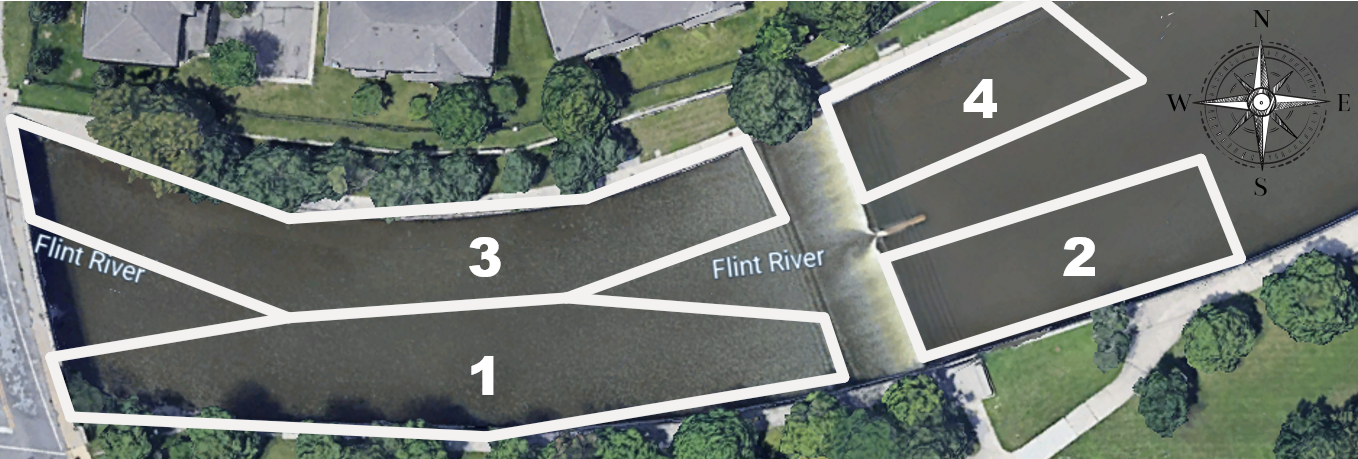
\includegraphics[width=\textwidth]{Img/Site_Map.png} \\
    \large
    \textbf{Site Map} \\
}
%%%%%%%%%%%%%%%%%%%%%%%%%%%%%%%%%%%%%%%%%%%%%%%%%%%%%%%%%%%%%%%%%%%%%%%%%%%%%%%%%%%%
%%% Diversity %%%%%%%%%%%%%%%%%%%%%%%%%%%%%%%%%%%%%%%%%%%%%%%%%%%%%%%%%%%%%%%%%%%%%%
%%%%%%%%%%%%%%%%%%%%%%%%%%%%%%%%%%%%%%%%%%%%%%%%%%%%%%%%%%%%%%%%%%%%%%%%%%%%%%%%%%%%
\headerbox{Diversity}{name=box10, column=1, row=0}{
  \begin{center}
    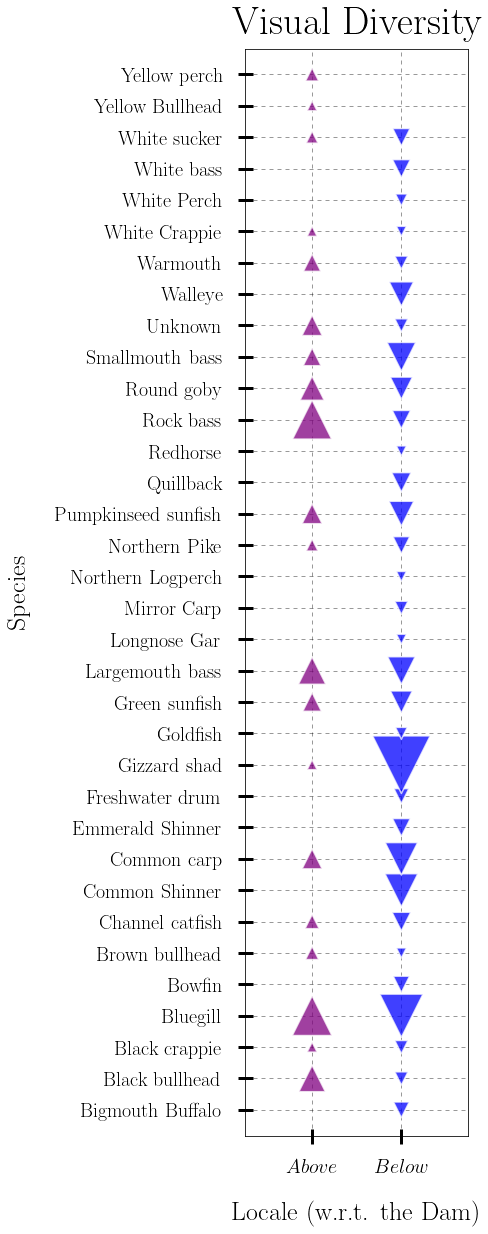
\includegraphics[width=.8\textwidth]{Img/Diversity_Bubble_Plot.png} \\
  \end{center}
  
  In this figure we compare catch rates between sites $1/3$ below the dam, and sites $2/4$ above the dam. 
  Notable differences show much higher catch rates of gizzard shad below the dam and rock bass above the dam.

}
%%%%%%%%%%%%%%%%%%%%%%%%%%%%%%%%%%%%%%%%%%%%%%%%%%%%%%%%%%%%%%%%%%%%%%%%%%%%%%%%%%%%
%%% Hg Compare %%%%%%%%%%%%%%%%%%%%%%%%%%%%%%%%%%%%%%%%%%%%%%%%%%%%%%%%%%%%%%%%%%%%%
%%%%%%%%%%%%%%%%%%%%%%%%%%%%%%%%%%%%%%%%%%%%%%%%%%%%%%%%%%%%%%%%%%%%%%%%%%%%%%%%%%%%
\headerbox{Toxins}{name=box20, column=2, row=0}{
  \begin{center}
    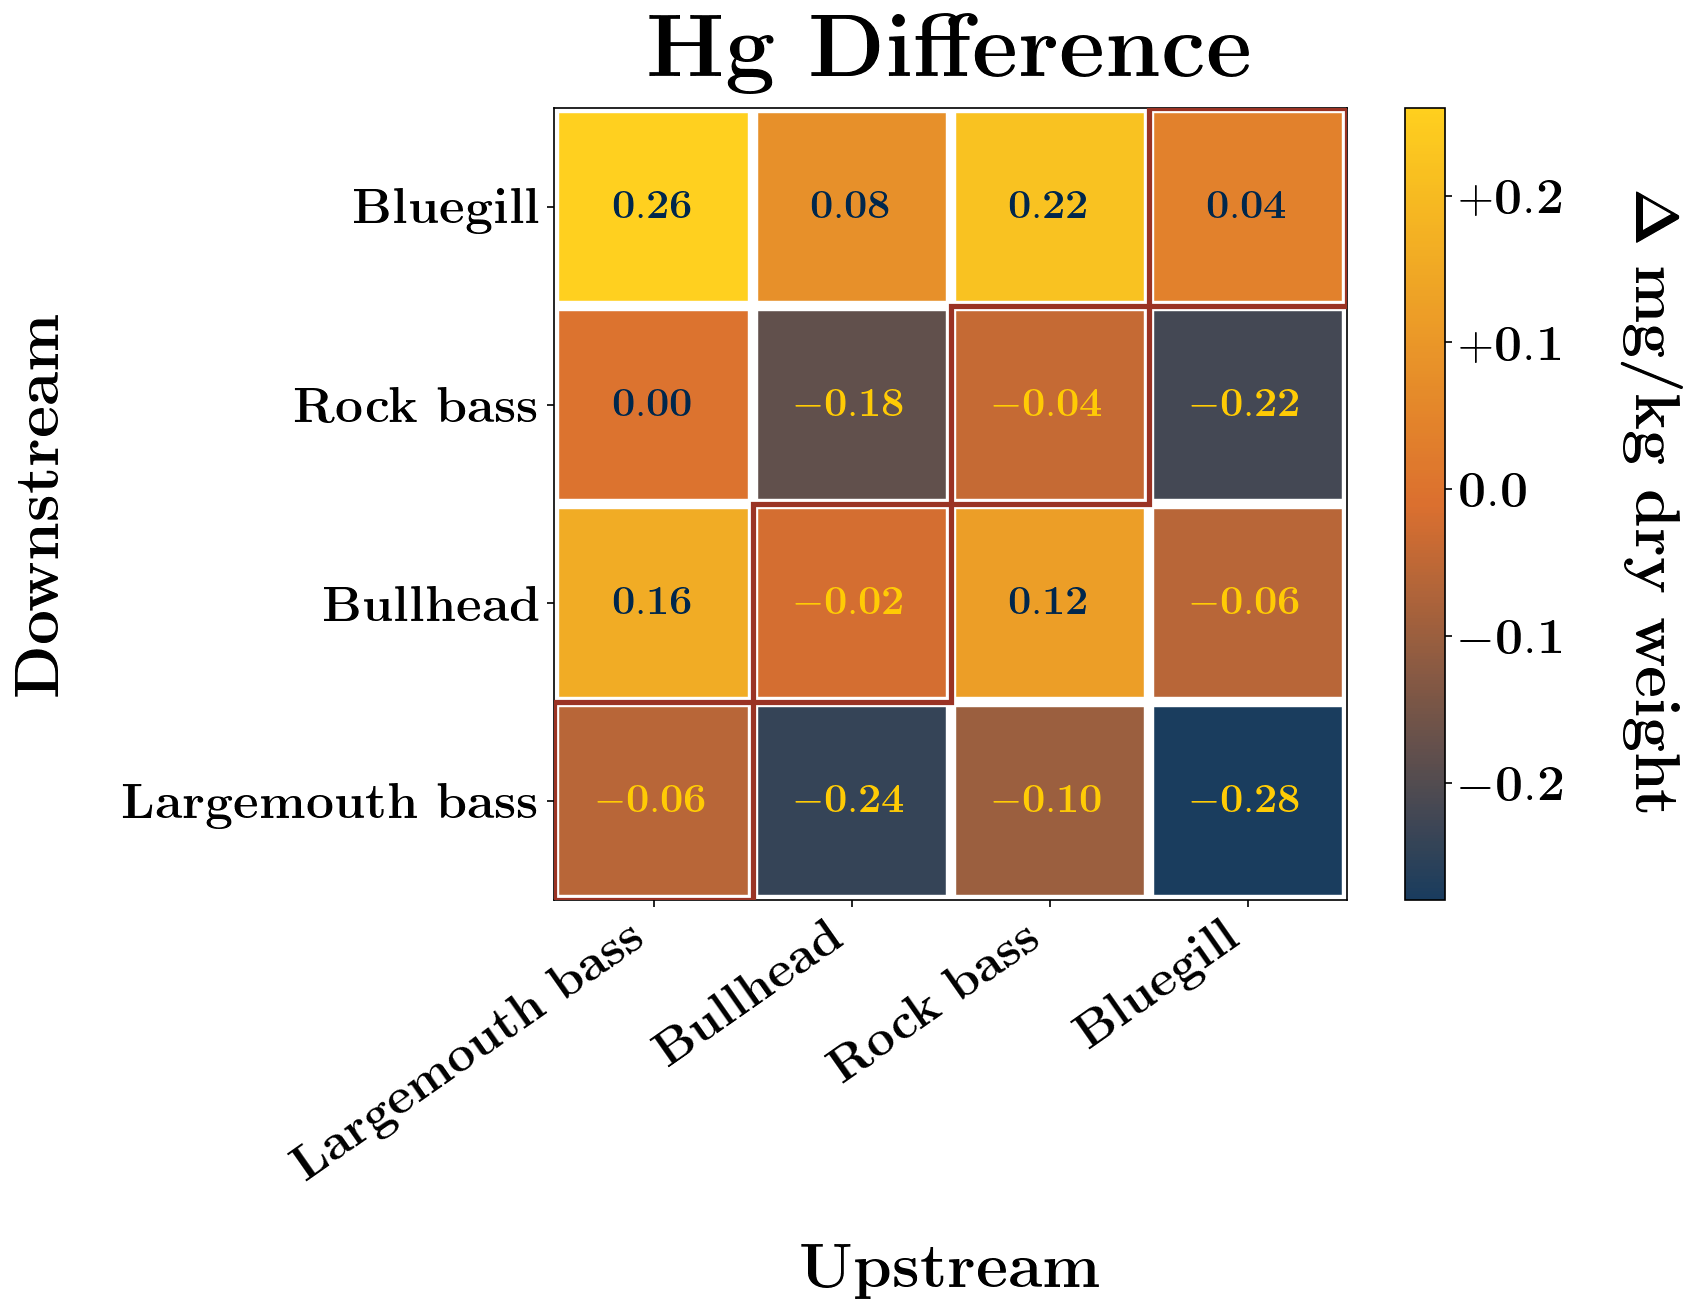
\includegraphics[width=.85\textwidth]{Img/Hg.png} \\
  \end{center}
  
  In this figure we compare Hg levels from tested fish caught between sites $1/3$ below the dam, and sites $2/4$ above the dam. 
  The values represent the difference between downstream and upstream species tested. \\ $(downstream - upstream)$.

}
%%%%%%%%%%%%%%%%%%%%%%%%%%%%%%%%%%%%%%%%%%%%%%%%%%%%%%%%%%%%%%%%%%%%%%%%%%%%%%%%%%%%
%%% Discussion %%%%%%%%%%%%%%%%%%%%%%%%%%%%%%%%%%%%%%%%%%%%%%%%%%%%%%%%%%%%%%%%%%%%%%%
%%%%%%%%%%%%%%%%%%%%%%%%%%%%%%%%%%%%%%%%%%%%%%%%%%%%%%%%%%%%%%%%%%%%%%%%%%%%%%%%%%%%
\headerbox{Discussion}{name=box21, column=2, row=1, below=box20}{

  \begin{itemize} \normalsize 
    \item Using Simpson's Diversity Index we compared species diversity above and below the dam. 
    We computed relative index values for the four sites $(S)$,  $D_{S_{3}} = 0.48 \le D_{S_{4}} = 0.72 \le D_{S_{1}} = 0.77 = D_{S_{2}} = 0.77$. \\
    \item Downstream yielded an index of 0.67 with 31 species caught. 
    The overall catch was dominated by Gizzard shad making it less even than upstream.
    \item Upstream yielded an index of 0.75 with 20 species caught. 
    Though there was less species diversity, it yielded a higher index because there was more eveness among the species caught.   
    \item The dam prevents species from traveling upstream, we caught more species below the dam. 
    Fishing methods upstream differed from downstream due to the different habitats. 
    This could impact the fish species caught and the quantities.
    \item Mercury levels were analyzed in fish above and below the dam.
    Bass contained higher levels of mercury compared to other species. 
    Fish higher in the trophic level bioaccumulate more than other species. 
    Downstream had more species with higher levels of mercury. 
    This could be due to downstream containing species that are migrating from The Great Lakes.
  \end{itemize}
}
%%%%%%%%%%%%%%%%%%%%%%%%%%%%%%%%%%%%%%%%%%%%%%%%%%%%%%%%%%%%%%%%%%%%%%%%%%%%%%%%%%%%
%%% Conclusion %%%%%%%%%%%%%%%%%%%%%%%%%%%%%%%%%%%%%%%%%%%%%%%%%%%%%%%%%%%%%%%%%%%%%
%%%%%%%%%%%%%%%%%%%%%%%%%%%%%%%%%%%%%%%%%%%%%%%%%%%%%%%%%%%%%%%%%%%%%%%%%%%%%%%%%%%%
\headerbox{Conclusion}{name=box30, column=3, row=0}{

  \textbf{
  The ecology study of the Flint River has been conducted for 2 years. 
  Study will be continued through the removal of the Hamilton Dam and restoration of the Flint River. 
  This pre-assessment will be used to compare data once restoration is 
  complete to understand how dam removal impacts riverine ecosystems.}
}
%%%%%%%%%%%%%%%%%%%%%%%%%%%%%%%%%%%%%%%%%%%%%%%%%%%%%%%%%%%%%%%%%%%%%%%%%%%%%%%%%%%%
%%% The Mitten %%%%%%%%%%%%%%%%%%%%%%%%%%%%%%%%%%%%%%%%%%%%%%%%%%%%%%%%%%%%%%%%%%%%%
%%%%%%%%%%%%%%%%%%%%%%%%%%%%%%%%%%%%%%%%%%%%%%%%%%%%%%%%%%%%%%%%%%%%%%%%%%%%%%%%%%%%
\headerbox{Where is Flint?}{name=box31, column=3, row=1, below=box30}{

  \begin{center}
    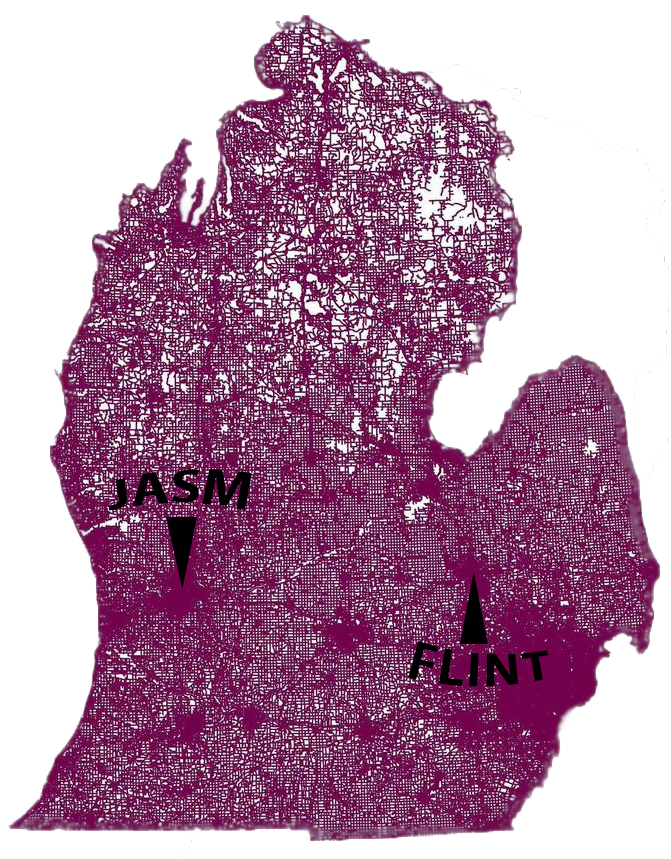
\includegraphics[width=0.55\textwidth]{Img/mit.png} \\
  \end{center}

}
%%%%%%%%%%%%%%%%%%%%%%%%%%%%%%%%%%%%%%%%%%%%%%%%%%%%%%%%%%%%%%%%%%%%%%%%%%%%%%%%%%%%
%%% Acknowledgements %%%%%%%%%%%%%%%%%%%%%%%%%%%%%%%%%%%%%%%%%%%%%%%%%%%%%%%%%%%%%%%
%%%%%%%%%%%%%%%%%%%%%%%%%%%%%%%%%%%%%%%%%%%%%%%%%%%%%%%%%%%%%%%%%%%%%%%%%%%%%%%%%%%%
\headerbox{Acknowledgements}{name=box32, column=3, row=2, below=box31}{

  We wold like to thank X ! Y ! Z !

  We would like to acknowledge our amazing mentor Dr. Heather Dawson

}
\end{poster}
\end{document}
